% =====================================================================
% File        : io_files_matlab.tex
% Deskripsi   : Slide Beamer (metropolis) — I/O Files MATLAB:
%               impor dan ekspor file (MAT, CSV/TXT, Excel, JSON, grafik)
% Proyek      : Basic MATLAB (ansyaku/matlab_doc)
% Penulis     : Andreas Syaloom Kurniawan
% Versi       : 1.1
% Dibuat      : 13 Oktober 2026
% Diperbarui  : 13 Oktober 2026 (slide Excel dipisah impor/ekspor)
% =====================================================================
\documentclass[10pt,aspectratio=169]{beamer}
\usetheme[progressbar=frametitle,numbering=fraction,block=fill]{metropolis}

% Dikompilasi dengan XeLaTeX (fontspec). Jika Fira Sans terpasang, metropolis memakainya otomatis.
\usepackage{fontspec}
\IfFontExistsTF{Fira Sans}{}{\setsansfont{Carlito}}
\setmonofont[Scale=0.88]{DejaVu Sans Mono}
\usepackage{booktabs}
\usepackage{array}
\usepackage{listings}
\usepackage{xcolor}
\usepackage{tikz}
\usetikzlibrary{arrows.meta,positioning,shapes.geometric}

% ---------- Warna ----------
\definecolor{kodebg}{RGB}{246,246,242}
\definecolor{kodekomentar}{RGB}{34,139,34}
\definecolor{kodestring}{RGB}{160,32,240}
\definecolor{kodekey}{RGB}{0,0,200}
\definecolor{aksen}{RGB}{235,129,27}
\definecolor{biru}{RGB}{35,55,59}
\definecolor{hijau}{RGB}{20,130,80}

% ---------- Listings gaya MATLAB ----------
\lstdefinestyle{matlab}{
  language=Matlab,
  basicstyle=\ttfamily\scriptsize,
  keywordstyle=\color{kodekey}\bfseries,
  commentstyle=\color{kodekomentar}\itshape,
  stringstyle=\color{kodestring},
  backgroundcolor=\color{kodebg},
  frame=single, rulecolor=\color{black!15},
  framesep=3pt, xleftmargin=4pt, xrightmargin=4pt,
  showstringspaces=false, columns=fullflexible, keepspaces=true,
  breaklines=true, upquote=true,
  morekeywords={table,dictionary,true,false},
  literate={…}{{\ldots}}1
}
\lstdefinestyle{plain}{
  basicstyle=\ttfamily\scriptsize,
  backgroundcolor=\color{black!3},
  frame=single, rulecolor=\color{black!15},
  framesep=3pt, xleftmargin=4pt, xrightmargin=4pt,
  columns=fullflexible, keepspaces=true, upquote=true
}
\lstset{style=matlab}
\newcommand{\kode}[1]{\texttt{\small #1}}

\title{I/O Files di MATLAB}
\subtitle{Impor dan Ekspor File: MAT, CSV/TXT, Excel, JSON, dan Grafik}
\author{Andreas Syaloom Kurniawan}
\institute{Basic MATLAB}
\date{Oktober 2026}

\begin{document}

\maketitle

% =====================================================================
\begin{frame}{Peta Materi}
  \setbeamertemplate{section in toc}[sections numbered]
  \tableofcontents
\end{frame}

% =====================================================================
\section{Mengapa I/O File?}

\begin{frame}{Apa itu I/O (Input/Output) file?}
  Variabel di Workspace MATLAB \alert{hilang} begitu MATLAB ditutup atau \kode{clear} dijalankan.
  Agar data dan hasil bisa dipakai lagi atau dibagikan, kita perlu \alert{membaca} dan \alert{menulis} file.

  \vspace{0.6em}
  \begin{center}
  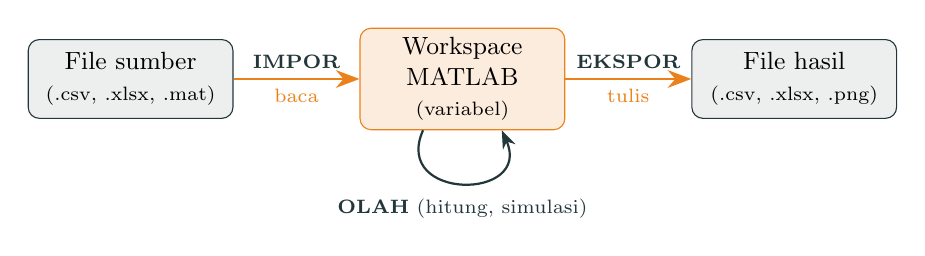
\begin{tikzpicture}[node distance=1.6cm,
      kotak/.style={draw=biru,fill=biru!8,rounded corners,minimum width=2.6cm,minimum height=1cm,align=center,font=\small},
      panah/.style={-{Stealth[length=3mm]},thick,aksen}]
    \node[kotak] (a) {File sumber\\\scriptsize(.csv, .xlsx, .mat)};
    \node[kotak,right=of a,fill=aksen!15,draw=aksen] (b) {Workspace\\MATLAB\\\scriptsize(variabel)};
    \node[kotak,right=of b] (c) {File hasil\\\scriptsize(.csv, .xlsx, .png)};
    \draw[panah] (a) -- node[above,font=\scriptsize,text=biru]{\textbf{IMPOR}} node[below,font=\scriptsize]{baca} (b);
    \draw[panah] (b) -- node[above,font=\scriptsize,text=biru]{\textbf{EKSPOR}} node[below,font=\scriptsize]{tulis} (c);
    \draw[thick,biru,-{Stealth}] ([xshift=-5mm]b.south) .. controls +(-0.4,-0.9) and +(0.4,-0.9) .. ([xshift=5mm]b.south);
    \node[below=0.75cm of b,font=\scriptsize,text=biru] {\textbf{OLAH} (hitung, simulasi)};
  \end{tikzpicture}
  \end{center}

  \vspace{0.4em}
  \begin{exampleblock}{Contoh nyata di ekonomi}
    Impor data PDB dan inflasi dari Excel (BPS/BI) $\rightarrow$ hitung pertumbuhan atau simulasi model
    $\rightarrow$ ekspor tabel hasil ke CSV dan grafik ke PNG untuk paper.
  \end{exampleblock}
\end{frame}

\begin{frame}{Dua kelompok fungsi yang perlu diingat}
  Hampir semua fungsi I/O di MATLAB berpasangan, dengan pola nama yang mudah ditebak:

  \vspace{0.6em}
  \begin{columns}[T]
    \begin{column}{0.47\textwidth}
      \begin{block}{Impor (membaca)}
        \kode{load}, \kode{readmatrix}, \kode{readtable}, \kode{readcell}, \kode{readlines}, \kode{fileread}, \kode{jsondecode}
      \end{block}
    \end{column}
    \begin{column}{0.47\textwidth}
      \begin{alertblock}{Ekspor (menulis)}
        \kode{save}, \kode{writematrix}, \kode{writetable}, \kode{writecell}, \kode{writelines}, \kode{fprintf}, \kode{jsonencode}
      \end{alertblock}
    \end{column}
  \end{columns}

  \vspace{0.8em}
  \textbf{Pola:} \kode{read}\textit{Jenis} $\leftrightarrow$ \kode{write}\textit{Jenis}.
  \textit{Jenis} menunjukkan \alert{bentuk data di MATLAB} (matrix, table, cell, lines), bukan format file.
  Format file ditentukan dari \alert{ekstensi} nama file.
\end{frame}

% =====================================================================
\section{Mengenal Jenis File MATLAB}

\begin{frame}{Ekstensi file utama MATLAB}
  \centering\small
  \begin{tabular}{>{\ttfamily}l l l}
    \toprule
    \textrm{\textbf{Ekstensi}} & \textbf{Isi} & \textbf{Kapan dipakai} \\
    \midrule
    .m      & Script atau function           & Program, fungsi, algoritma \\
    .mlx    & Live Script (kode + teks + grafik) & Analisis, belajar, laporan \\
    .mat    & Variabel/data MATLAB           & Menyimpan data apa adanya \\
    .fig    & Figure (grafik yang bisa diedit) & Menyimpan grafik untuk diubah lagi \\
    .mlapp  & Aplikasi App Designer          & GUI dengan tombol, slider \\
    .p      & P-code (kode tersembunyi)      & Membagikan kode tanpa isi sumber \\
    .slx    & Model Simulink                 & Simulasi berbasis blok \\
    .mdl    & Model Simulink format lama     & File Simulink versi lama \\
    .mex*   & MEX (C/C++/Fortran terkompilasi) & Mempercepat bagian kode berat \\
    \bottomrule
  \end{tabular}

  \vspace{0.6em}
  \raggedright\footnotesize
  Akhiran MEX bergantung platform: \kode{.mexw64} (Windows), \kode{.mexa64} (Linux), \kode{.mexmaci64}/\kode{.mexmaca64} (macOS Intel/Apple Silicon).
\end{frame}

\begin{frame}[fragile]{Script (.m) vs Live Script (.mlx)}
  Kodenya \alert{bisa sama persis}. Yang berbeda adalah \alert{cara menyajikan hasil}.
  \vspace{0.3em}
\begin{lstlisting}
x = 0:0.1:10;
y = sin(x);
plot(x, y); title('Grafik Sinus');
\end{lstlisting}
  \begin{columns}[T]
    \begin{column}{0.47\textwidth}
      \begin{block}{Script \kode{.m}}
        \small Output teks muncul di \textit{Command Window}, grafik di jendela \textit{Figure} terpisah.
        Cocok untuk fungsi dan program modular.
      \end{block}
    \end{column}
    \begin{column}{0.47\textwidth}
      \begin{block}{Live Script \kode{.mlx}}
        \small Kode, output, grafik, teks, dan rumus berada dalam \alert{satu dokumen}.
        Bisa diekspor ke PDF/HTML/Word dari Live Editor.
      \end{block}
    \end{column}
  \end{columns}
  \vspace{0.4em}
  \footnotesize\textbf{Analogi:} Live Script $\approx$ \alert{Jupyter Notebook}, bukan dashboard.
  Untuk dashboard interaktif (slider, tombol) gunakan \textbf{App Designer} (\kode{.mlapp}).
\end{frame}

% =====================================================================
\section{Persiapan: Folder Kerja}

\begin{frame}[fragile]{Di mana MATLAB mencari dan menyimpan file?}
  Jika nama file ditulis \alert{tanpa folder}, MATLAB membaca/menulis di \alert{Current Folder}.
  Banyak error ``file not found'' berasal dari sini.
\begin{lstlisting}
pwd                          % tampilkan folder kerja sekarang
cd('D:\kuliah\matlab')       % pindah folder kerja (contoh Windows)
dir                          % daftar file di folder kerja

% Cara aman: susun path lengkap dengan fullfile
folderData = fullfile(pwd, 'data');
if ~exist(folderData, 'dir')
    mkdir(folderData);       % buat folder jika belum ada
end
namaFile = fullfile(folderData, 'hasil.csv');
\end{lstlisting}
  \begin{exampleblock}{Tips}
    \kode{fullfile} otomatis memakai pemisah folder yang benar (\kode{\textbackslash} di Windows, \kode{/} di macOS/Linux),
    sehingga kode Anda jalan di komputer mana pun.
  \end{exampleblock}
\end{frame}

\begin{frame}{Format apa, fungsi apa? (peta besar)}
  \centering\footnotesize
  \begin{tabular}{l l l l}
    \toprule
    \textbf{Format} & \textbf{Impor} & \textbf{Ekspor} & \textbf{Cocok untuk} \\
    \midrule
    \texttt{.mat}  & \texttt{load}       & \texttt{save}         & Semua variabel MATLAB, apa adanya \\
    \texttt{.csv}  & \texttt{readmatrix}, \texttt{readtable} & \texttt{writematrix}, \texttt{writetable} & Data tabel lintas aplikasi \\
    \texttt{.txt}  & \texttt{readtable}, \texttt{readlines} & \texttt{writetable}, \texttt{writelines} & Teks atau data ber-delimiter \\
    \texttt{.xlsx} & \texttt{readtable}, \texttt{readmatrix} & \texttt{writetable}, \texttt{writematrix} & Dibagikan ke pengguna Excel \\
    \texttt{.json} & \texttt{jsondecode} & \texttt{jsonencode} & Python, web, API \\
    \texttt{.png}, \texttt{.pdf} & -- & \texttt{exportgraphics} & Grafik untuk paper/slide \\
    \texttt{.fig}  & \texttt{openfig} & \texttt{savefig} & Grafik yang masih bisa diedit \\
    \bottomrule
  \end{tabular}

  \vspace{0.8em}
  \raggedright\small
  Kita akan bahas satu per satu, \alert{mulai dari yang paling sederhana}: satu angka, lalu vektor, matriks, dan tabel.
\end{frame}

% =====================================================================
\section{File .mat: Format Asli MATLAB}

\begin{frame}[fragile]{Konsep: \kode{save} dan \kode{load}}
  File \kode{.mat} adalah ``kotak penyimpanan'' khusus MATLAB.
  Variabel disimpan \alert{lengkap dengan nama dan tipenya}, lalu bisa dikembalikan persis sama.

  \vspace{0.3em}
  \textbf{Mulai dari satu angka (skalar):}
\begin{lstlisting}
r = 0.0575;                  % suku bunga, satu angka
save('bunga.mat', 'r');      % simpan variabel r ke file bunga.mat

clear r                      % hapus r dari Workspace
load('bunga.mat');           % r muncul kembali
disp(r)                      % 0.0575
\end{lstlisting}
  \begin{alertblock}{Perhatikan}
    Nama variabel ditulis sebagai \alert{teks dalam tanda kutip} (\kode{'r'}), bukan \kode{r}.
    Tanpa nama variabel, \kode{save('bunga.mat')} menyimpan \alert{seluruh} isi Workspace.
  \end{alertblock}
\end{frame}

\begin{frame}[fragile]{\kode{.mat}: beberapa variabel sekaligus}
\begin{lstlisting}
tahun   = (2015:2024)';                  % vektor kolom
inflasi = [3.4 3.0 3.6 3.1 2.7 1.7 1.9 5.5 2.6 1.6]';
info    = 'Inflasi tahunan (persen)';    % teks

save('makro.mat', 'tahun', 'inflasi', 'info');   % simpan tiga variabel
whos('-file', 'makro.mat')                       % intip isi tanpa memuat

kurs = 15500;
save('makro.mat', 'kurs', '-append');            % tambah tanpa menimpa
\end{lstlisting}
  \textbf{Cara memuat yang lebih rapi: ke dalam struct}
\begin{lstlisting}
S = load('makro.mat');       % semua variabel masuk ke struct S
S.inflasi                    % akses dengan titik
x = load('makro.mat', 'tahun');   % hanya memuat variabel tahun
\end{lstlisting}
  \footnotesize Memuat ke struct mencegah variabel di Workspace \alert{tertimpa diam-diam} oleh variabel bernama sama di file.
  Data sangat besar ($>$2 GB) simpan dengan opsi \kode{'-v7.3'}.
\end{frame}

% =====================================================================
\section{Teks dan CSV}

\begin{frame}{Konsep: apa itu file CSV?}
  CSV (\textit{Comma-Separated Values}) adalah \alert{file teks biasa}: setiap baris = satu observasi,
  kolom dipisahkan \alert{delimiter} (koma, titik koma, atau tab).
  \vspace{0.5em}
  \begin{columns}[T]
    \begin{column}{0.45\textwidth}
      \textbf{Isi file \kode{inflasi.csv}} \\[0.2em]
      \ttfamily\small
      \colorbox{kodebg}{\parbox{0.9\linewidth}{
      Tahun,Inflasi\\
      2022,5.51\\
      2023,2.61\\
      2024,1.57}}
    \end{column}
    \begin{column}{0.5\textwidth}
      \begin{block}{Kenapa CSV populer?}
        \small
        \begin{itemize}
          \item Bisa dibuka Excel, R, Python, Stata, bahkan Notepad.
          \item Ringan dan tidak bergantung versi software.
          \item Kekurangan: hanya menyimpan angka/teks, \alert{tanpa} format, rumus, atau tipe data khusus.
        \end{itemize}
      \end{block}
    \end{column}
  \end{columns}
  \vspace{0.4em}
  \small \kode{.txt} sama saja secara prinsip; bedanya hanya ekstensi dan biasanya delimiter (sering tab).
\end{frame}

\begin{frame}[fragile]{Ekspor angka: \kode{writematrix}}
  Untuk data yang \alert{semuanya angka} (skalar, vektor, matriks), gunakan \kode{writematrix}.
\begin{lstlisting}
a = 7;                           % 1) skalar
writematrix(a, 'skalar.csv');    %    file berisi: 7

v = [10 20 30];                  % 2) vektor baris
writematrix(v, 'vektor.csv');    %    file berisi: 10,20,30

A = [1 2 3; 4 5 6];              % 3) matriks 2x3
writematrix(A, 'matriks.csv');   %    dua baris, tiga kolom
writematrix(A, 'matriks.txt', 'Delimiter', 'tab');   % pakai tab
\end{lstlisting}
  \textbf{Impor kembali:}
\begin{lstlisting}
B = readmatrix('matriks.csv')    % B sama dengan A
isequal(A, B)                    % 1 (true)
\end{lstlisting}
\end{frame}

\begin{frame}[fragile]{Ekspor tabel: \kode{writetable}}
  Data ekonomi biasanya punya \alert{nama kolom} (Tahun, PDB, Inflasi). Untuk itu gunakan \kode{table}.
\begin{lstlisting}
Tahun   = (2022:2024)';
Inflasi = [5.51; 2.61; 1.57];
T = table(Tahun, Inflasi);       % nama kolom diambil dari nama variabel

writetable(T, 'inflasi.csv');                       % CSV dengan header
writetable(T, 'inflasi.txt', 'Delimiter', '\t');    % teks, dipisah tab
\end{lstlisting}
  \textbf{Impor kembali:}
\begin{lstlisting}
T2 = readtable('inflasi.csv');
T2.Inflasi                       % akses kolom dengan nama
mean(T2.Inflasi)                 % langsung bisa dihitung
\end{lstlisting}
  \begin{block}{Aturan praktis}
    \small Angka saja $\rightarrow$ \kode{writematrix}/\kode{readmatrix}. \quad
    Ada nama kolom atau campuran angka-teks $\rightarrow$ \kode{writetable}/\kode{readtable}.
  \end{block}
\end{frame}

\begin{frame}[fragile]{Jebakan umum saat impor CSV}
  \begin{enumerate}
    \item \textbf{Desimal koma.} Excel berbahasa Indonesia sering menulis \kode{5,51} dan memakai \kode{;} sebagai delimiter.
\begin{lstlisting}
T = readtable('data_id.csv', 'Delimiter', ';', 'DecimalSeparator', ',');
\end{lstlisting}
    \item \textbf{Nama kolom berubah.} Header seperti \kode{PDB (miliar)} diubah agar jadi nama variabel valid. Agar tetap asli:
\begin{lstlisting}
T = readtable('data.csv', 'VariableNamingRule', 'preserve');
T.("PDB (miliar)")               % akses nama kolom ber-spasi
\end{lstlisting}
    \item \textbf{Header ikut terbaca sebagai data.} Periksa dengan \kode{head(T)} dan \kode{summary(T)} setelah impor.
    \item \textbf{File tertimpa.} \kode{write*} menimpa file lama \alert{tanpa peringatan}. Gunakan nama file berbeda atau cek dengan \kode{exist}.
  \end{enumerate}
\end{frame}

\begin{frame}[fragile]{Teks bebas: \kode{writelines}, \kode{readlines}, \kode{fprintf}}
  Kadang yang ingin disimpan bukan tabel, melainkan \alert{kalimat atau laporan singkat}.
\begin{lstlisting}
% Cara sederhana (R2022a ke atas)
baris = ["Laporan simulasi"; "Rata-rata inflasi: 3.23 persen"];
writelines(baris, 'laporan.txt');
isi = readlines('laporan.txt')        % string array, satu elemen per baris

% Cara klasik (semua versi): buka - tulis - tutup
rataan = mean([5.51 2.61 1.57]);
fid = fopen('laporan2.txt', 'w');     % 'w' = write (timpa), 'a' = append
fprintf(fid, 'Rata-rata inflasi: %.2f persen\n', rataan);
fclose(fid);                          % WAJIB ditutup
\end{lstlisting}
  \footnotesize \kode{\%.2f} artinya angka desimal dua digit, \kode{\textbackslash n} artinya pindah baris.
  Lupa \kode{fclose} bisa membuat file terkunci atau isinya tidak lengkap.
\end{frame}

% =====================================================================
\section{Excel}

\begin{frame}[fragile]{Ekspor ke Excel (\kode{.xlsx})}
  Fungsinya \alert{sama dengan CSV}; cukup ganti ekstensi menjadi \kode{.xlsx}.
  Bonus Excel: kita bisa memilih \textit{sheet} dan sel awal.

  \centering\footnotesize
  \begin{tabular}{l l l}
    \toprule
    \textbf{Data di MATLAB} & \textbf{Fungsi ekspor} & \textbf{Hasil di Excel} \\
    \midrule
    Tabel (\kode{table}) & \texttt{writetable(T, 'f.xlsx')}  & Baris 1 = nama kolom, di bawahnya data \\
    Matriks/vektor angka & \texttt{writematrix(A, 'f.xlsx')} & Angka saja, tanpa header \\
    \bottomrule
  \end{tabular}
  \raggedright
\begin{lstlisting}
Tahun = (2022:2024)';  Inflasi = [5.51; 2.61; 1.57];
T = table(Tahun, Inflasi);           % tabel: punya nama kolom
A = [1 2 3; 4 5 6];                  % matriks: angka saja

writetable(T, 'hasil.xlsx', 'Sheet', 'Inflasi');                 % tabel ke sheet "Inflasi"
writetable(T, 'hasil.xlsx', 'Sheet', 'Inflasi2', 'Range', 'B3'); % mulai dari sel B3
writematrix(A, 'hasil.xlsx', 'Sheet', 'Matriks');                % matriks ke sheet lain
\end{lstlisting}
  \begin{alertblock}{Ingat}
    \small Satu file bisa berisi banyak sheet. MATLAB hanya menulis \alert{nilai}, bukan format sel, warna, atau rumus.
    Tutup file di Excel sebelum menulis ke file yang sama.
  \end{alertblock}
\end{frame}

\begin{frame}[fragile]{Impor dari Excel (\kode{.xlsx})}
  Sebelum mengimpor, tanyakan: \alert{apakah sheet itu punya baris header (nama kolom)?}

  \centering\footnotesize
  \begin{tabular}{l l l}
    \toprule
    \textbf{Isi sheet Excel} & \textbf{Fungsi impor} & \textbf{Hasil di MATLAB} \\
    \midrule
    Ada header (nama kolom)   & \texttt{T = readtable('f.xlsx')}  & \kode{table}; kolom diakses \kode{T.Nama} \\
    Angka saja, tanpa header  & \texttt{A = readmatrix('f.xlsx')} & Matriks \kode{double}; header teks jadi \kode{NaN} \\
    \bottomrule
  \end{tabular}
  \raggedright
\begin{lstlisting}
sheetnames('hasil.xlsx')                          % 1) cek dulu: ada sheet apa saja?

T2 = readtable('hasil.xlsx', 'Sheet', 'Inflasi'); % 2) sheet ber-header -> tabel
mean(T2.Inflasi)                                  %    langsung bisa dihitung

A2 = readmatrix('hasil.xlsx', 'Sheet', 'Matriks'); % 3) angka saja -> matriks
B  = readmatrix('hasil.xlsx', 'Sheet', 'Matriks', ...
                'Range', 'A1:B2');                 %    hanya sebagian sel
\end{lstlisting}
  \begin{exampleblock}{Tips}
    \small Tanpa opsi \kode{'Sheet'}, MATLAB membaca \alert{sheet pertama}.
    Setelah impor, selalu periksa hasilnya dengan \kode{head(T2)} atau \kode{size(A2)}.
  \end{exampleblock}
\end{frame}

% =====================================================================
\section{Struktur Data dan JSON}

\begin{frame}[fragile]{Array, matrix, dictionary: apa bedanya?}
  \begin{itemize}
    \item \textbf{Array}: kumpulan elemen dalam susunan tertentu (1D, 2D, $n$D).
    \item \textbf{Matrix}: array \alert{2 dimensi}, umumnya untuk hitungan numerik.
    \item \textbf{Dictionary}: pasangan \alert{key--value}; elemen diakses lewat kunci, bukan posisi (R2022b ke atas).
  \end{itemize}
\begin{lstlisting}
A = [10 20 30; 40 50 60];              % array 2D = matrix
D = dictionary(["IDN","MYS","THA"], [1.57 1.80 0.40]);   % negara -> inflasi
D("IDN")                               % 1.5700
\end{lstlisting}
  \textbf{Mengekspor dictionary:} paling aman ke \kode{.mat}. Untuk CSV/Excel, ubah dulu menjadi tabel:
\begin{lstlisting}
save('dict.mat', 'D');                               % struktur tetap utuh
Td = table(keys(D), values(D), 'VariableNames', {'Negara','Inflasi'});
writetable(Td, 'dict.csv');
\end{lstlisting}
\end{frame}

\begin{frame}[fragile]{JSON: \kode{jsonencode} dan \kode{jsondecode}}
  JSON adalah format teks terstruktur yang dipakai Python, JavaScript, dan API web.
  Fungsinya \alert{bawaan (native)} MATLAB, tanpa library tambahan.
  \vspace{0.2em}
  \begin{columns}[T]
    \begin{column}{0.55\textwidth}
\begin{lstlisting}
% 1) matriks -> JSON
A = [1 2 3; 4 5 6];
txt = jsonencode(A)    % '[[1,2,3],[4,5,6]]'

% 2) struct -> JSON (paling alami)
s.negara  = "Indonesia";
s.tahun   = 2024;
s.inflasi = 1.57;
txt = jsonencode(s, 'PrettyPrint', true);
writelines(txt, 'data.json');

% 3) baca kembali
s2 = jsondecode(fileread('data.json'));
s2.inflasi             % 1.5700
\end{lstlisting}
    \end{column}
    \begin{column}{0.42\textwidth}
      \textbf{Isi \kode{data.json}} \\[0.2em]
\begin{lstlisting}[style=plain]
{
  "negara": "Indonesia",
  "tahun": 2024,
  "inflasi": 1.57
}
\end{lstlisting}
      \begin{alertblock}{Batasan}
        \footnotesize JSON tidak menjamin tipe data MATLAB terjaga persis (mis.\ \kode{int8}, kompleks, dimensi).
        Dukungan tabel/dictionary bergantung versi: cek dokumentasi versi Anda.
      \end{alertblock}
    \end{column}
  \end{columns}
\end{frame}

% =====================================================================
\section{Mengekspor Grafik}

\begin{frame}[fragile]{Grafik: gambar statis vs figure yang bisa diedit}
\begin{lstlisting}
tahun = 2015:2024;
inflasi = [3.4 3.0 3.6 3.1 2.7 1.7 1.9 5.5 2.6 1.6];
plot(tahun, inflasi, '-o'); grid on
xlabel('Tahun'); ylabel('Inflasi (%)'); title('Inflasi Indonesia');

exportgraphics(gcf, 'inflasi.png', 'Resolution', 300);   % gambar untuk slide
exportgraphics(gcf, 'inflasi.pdf', 'ContentType', 'vector');  % vektor untuk paper
savefig(gcf, 'inflasi.fig');                               % masih bisa diedit
openfig('inflasi.fig');                                    % buka lagi
\end{lstlisting}
  \begin{columns}[T]
    \begin{column}{0.48\textwidth}
      \begin{block}{PNG vs PDF}
        \small PNG = piksel (pecah bila diperbesar). PDF vektor = tetap tajam; ideal untuk LaTeX.
      \end{block}
    \end{column}
    \begin{column}{0.48\textwidth}
      \begin{block}{\kode{gcf} dan \kode{gca}}
        \small \kode{gcf} = seluruh figure, \kode{gca} = sumbu (axes) yang aktif saja.
      \end{block}
    \end{column}
  \end{columns}
\end{frame}

% =====================================================================
\section{Jembatan ke R dan Python}

\begin{frame}[fragile]{Membawa hasil MATLAB ke R (.RData) dan Python}
  MATLAB tidak menulis \kode{.RData} secara langsung. Jalur paling sederhana: \alert{lewat CSV}.
  \vspace{0.2em}
  \begin{columns}[T]
    \begin{column}{0.48\textwidth}
      \textbf{Di MATLAB}
\begin{lstlisting}
writetable(T, 'hasil.csv');
\end{lstlisting}
      \textbf{Di R}
\begin{lstlisting}[style=plain]
data <- read.csv("hasil.csv")
save(data, file = "hasil.RData")
\end{lstlisting}
    \end{column}
    \begin{column}{0.48\textwidth}
      \textbf{Di Python (pandas)}
\begin{lstlisting}[style=plain]
import pandas as pd
data = pd.read_csv("hasil.csv")
\end{lstlisting}
      \textbf{Alternatif tanpa CSV}
      \begin{itemize}\small
        \item R: paket \kode{R.matlab}, fungsi \kode{readMat()}.
        \item Python: \kode{scipy.io.loadmat()}.
        \item Keduanya untuk \kode{.mat} versi lama; file \kode{-v7.3} (berbasis HDF5) perlu \kode{h5py}/\kode{rhdf5}.
      \end{itemize}
    \end{column}
  \end{columns}
\end{frame}

% =====================================================================
\section{Ringkasan dan Latihan}

\begin{frame}{Ringkasan: pilih format berdasarkan tujuan}
  \centering\small
  \begin{tabular}{l l l}
    \toprule
    \textbf{Tujuan} & \textbf{Format} & \textbf{Fungsi} \\
    \midrule
    Lanjut kerja besok di MATLAB        & \kode{.mat}  & \kode{save} / \kode{load} \\
    Data angka murni                    & \kode{.csv}  & \kode{writematrix} / \kode{readmatrix} \\
    Data dengan nama kolom              & \kode{.csv}, \kode{.xlsx} & \kode{writetable} / \kode{readtable} \\
    Dibagikan ke pengguna Excel         & \kode{.xlsx} & \kode{writetable} (+ \kode{'Sheet'}) \\
    Dipakai Python, web, API            & \kode{.json} & \kode{jsonencode} / \kode{jsondecode} \\
    Catatan atau laporan teks           & \kode{.txt}  & \kode{writelines}, \kode{fprintf} \\
    Grafik untuk paper/slide            & \kode{.pdf}, \kode{.png} & \kode{exportgraphics} \\
    Grafik yang mau diedit lagi         & \kode{.fig}  & \kode{savefig} / \kode{openfig} \\
    Dokumentasi analisis lengkap        & \kode{.mlx} $\rightarrow$ PDF & Export di Live Editor \\
    \bottomrule
  \end{tabular}
\end{frame}

\begin{frame}{Latihan}
  \begin{enumerate}
    \item Buat skalar \kode{g = 5.05} (pertumbuhan PDB). Simpan ke \kode{pdb.mat}, hapus dari Workspace, lalu muat kembali ke struct.
    \item Buat matriks $3\times 2$ berisi angka bebas. Ekspor ke \kode{latihan.csv}, impor lagi, lalu buktikan dengan \kode{isequal} bahwa hasilnya sama.
    \item Buat tabel berisi kolom \kode{Tahun} (2020--2024) dan \kode{Kurs}. Ekspor ke Excel pada sheet \kode{"Kurs"} mulai sel \kode{B2}.
    \item Buat struct berisi nama provinsi, tahun, dan IPM. Ubah ke JSON dengan \kode{PrettyPrint}, simpan, lalu baca kembali.
    \item Plot data kurs dari soal 3, simpan sebagai PDF vektor dan sebagai \kode{.fig}.
  \end{enumerate}
  \vspace{0.5em}
  \begin{exampleblock}{Tantangan}
    Impor sebuah CSV ber-desimal koma dan delimiter \kode{;} (format Excel Indonesia), hitung rata-rata kolomnya,
    lalu tulis hasilnya ke \kode{laporan.txt} dengan \kode{fprintf}.
  \end{exampleblock}
\end{frame}

\begin{frame}[standout]
  Terima kasih \\[0.5em]
  \normalsize Pertanyaan dan diskusi
\end{frame}

\end{document}
